\chapter{Opis projektnog zadatka}
		
		%\textbf{\textit{dio 1. revizije}}\\
		
		%\textit{Na osnovi projektnog zadatka detaljno opisati korisničke zahtjeve. Što jasnije opisati cilj projektnog zadatka, razraditi problematiku zadatka, dodati nove aspekte problema i potencijalnih rješenja. Očekuje se minimalno 3, a poželjno 4-5 stranica opisa.	Teme koje treba dodatno razraditi u ovom poglavlju su:}
		%\begin{packed_item}
			%\item \textit{potencijalna korist ovog projekta}
			%\item \textit{postojeća slična rješenja (istražiti i ukratko opisati razlike u odnosu na zadani zadatak). Dodajte slike koja predočavaju slična rješenja.}
			%\item \textit{skup korisnika koji bi mogao biti zainteresiran za ostvareno rješenje.}
			%\item \textit{mogućnost prilagodbe rješenja }
			%\item \textit{opseg projektnog zadatka}
			%\item \textit{moguće nadogradnje projektnog zadatka}
		%\end{packed_item}
		
		%\textit{Za pomoć pogledati reference navedene u poglavlju „Popis literature“, a po potrebi konzultirati sadržaj na internetu koji nudi dobre smjernice u tom pogledu.}

		Cilj je projektnog zadatka razviti web-aplikaciju koja bi sudionicima stručne konferencije poboljšala ukupan doživljaj konferencije te im raznim funkcionalnostima olakšala prisustvovanje. Funkcionalnosti koje bi omogućile izvrsno korisničko iskustvo su mogućnost direktnog video praćenja konferencije u glavnoj konferencijskoj dvorani, dio s informacijama o mjestu održavanja konferencije koji između ostalog sadrži podatke o trenutnim vremenskim uvjetima i vremenskoj prognozi za navedenu lokaciju, pregled fotografija s konferencije i lokalno pohranjivanje na vlastiti uređaj te pregled i korištenje promotivnih materijala pokrovitelja. Među istaknutim je funkcionalnostima pregled radova - postera ili prezentacija - ostalih sudionika i mogućnost ocjenjivanja onog rada za kojeg smatraju da je najbolji. Budući da organizatori stručnih konferencija ciljaju na što veći broj sudionika, razvojem aplikacije svakako bi postigli veći doseg jer bi se konferenciji moglo priključiti s bilo koje lokacije i u bilo kojem vremenu unutar ukupnog trajanja konferencije.\\
		
		Sistemski administrator zadužen je za proces prijave odnosno on prijavljuje autore i njihove radove nakon što mu autori koji sudjeluju na stručnoj konferenciji elektroničkom poštom pošalju sve potrebne materijale te bira fotografije koje će biti dostupne za pregledavanje i preuzimanje na aplikaciji. Sistemski administrator može definirati sve potrebne uvjete za ispravan rad sustava.\\
		
		Prilikom dolaska na stručnu konferenciju sudionici prijavljuju svoj dolazak te pritom dobivaju lozinku za pristup toj određenoj stručnoj konferenciji na web-aplikaciji. Ukoliko sudionik odluči koristiti web-aplikaciju pri njenom otvaranju unosi lozinku koju je dobio jer je ona jedinstveni identifikator konferencije koju je posjetio. Nakon unosa lozinke prikazuju mu se svi stručni radovi (nema mogućnost glasanja) te mu se nudi mogućnost samostalne registracije u sustav kako bi mogao pristupiti svim funkcionalnostima i pogodnostima aplikacije.\\\\

        \textbf{Za samostalnu registraciju u sustav potrebno je sljedeće:}
        \begin{itemize}
        	\item \textit{Ime}
        	\item \textit{Prezime}
        	\item \textit{Adresa elektroničke pošte}
        	\item \textit{Lozinka}
        \end{itemize}

		\textbf{Za prijavu u sustav potrebno je sljedeće:}
        \begin{itemize}
            \item \textit{Adresa elektroničke pošte}
            \item \textit{Lozinka}
        \end{itemize}
        
        \textbf{Nakon registracije u sustav korisniku je dostupno sljedeće:}
        \begin{itemize}
        	\item \textit{Direktno video praćenje trenutnih događanja u glavnoj konferencijskoj dvorani}
        	\item \textit{Prikaz svih prijavljenih radova}
        	\item \textit{Glasanje za najbolji rad po vlastitom izboru unutar vremenskog okvira}
        	\item \textit{Izabrane fotografije s konferencije koje je moguće preuzeti na vlastiti uređaj}
        	\item \textit{Promotivni materijali pokrovitelja konferencije}
        	\item \textit{Prikaz informacija o mjestu održavanja konferencije i podatci o trenutnim vremenskim uvjetima i vremenskoj prognozi za navedenu lokaciju}
        	\item \textit{Rezultati glasovanja za najbolji poster (\underbar{nakon završetka glasovanja})}
        \end{itemize}

		Sudionici stručne konferencije tijekom određenog vremenskog razdoblja koje je određeno danima i vremenom održavanja konferencije mogu glasovati za rad koji predstavlja pojedinog predavača na konferenciji. Svi radovi prikazani su u web-aplikaciji. Svaki sudionik može glasovati samo jednom odnosno za samo jedan rad za kojeg smatra da je najbolji. Ukoliko se sudionik predomisli te želi dati glas drugom radu to može učiniti ukoliko to odluči dok glasovanje još traje. Po završetku glasovanja objavljuju se rezultati koji su dostupni svim registriranim korisnicima i šalje se obavijest autorima o rangu njihovog rada prema glasovima sudionika. Porukom elektroničke pošte na dodjelu nagrade poziva se autore prva tri rada s najviše glasova, a sve se ostale sudionike također elektroničkom poštom obavještava o mjestu i vremenu dodjele nagrade. Nakon završetka glasovanja rezultati se objavljuju na web-aplikaciji u obliku rang tablice.\\
		
		Aplikacija bi bila od velikog značaja za sve organizatore stručnih konferencija, znanstveno-istraživačkih skupova i raznih drugih javnih događanja jer uvelike olakšava organizaciju i komunikaciju sa sudionicima. Sve informacije sudionici bi mogli dobivati preko aplikacije, a ukoliko ne bi mogli prisustvovati uživo mogli bi se uključiti u direktne videoprijenose čime bi se omogućio puno veći broj posjetitelja konferencije te bi njen značaj mogao brzo rasti među željenim krugovima ljudi.\\
		
		Budući da bi aplikaciju koristio vrlo velik broj ljudi te bi ona uključivala video prijenos uživo potrebno je osigurati stabilnost i brzinu aplikacije kako bi svaki pojedinac mogao u trenutku pristupiti željenom sadržaju i ostao zadovoljan korisničkim iskustvom. Razvojni programeri stoga moraju računati na to da bi moglo biti problema s prekapacitiranošću i unaprijed takve probleme pokušati suzbiti kako ne bi došlo do rušenja aplikacije. Osim toga, aplikacija sadrži bazu s puno osobnih podataka te treba osigurati odgovarajuću zaštitu kako podaci ne bi iscurili pa da se ne naruši privatnost korisnika ili još opasnije - da ne bi bili zlouporabljeni. Zadatak organizatora bio bi osigurati stabilnu mrežu odnosno Wi-Fi na cijelom području održavanja konferencije kako bi se aplikacija mogla nesmetano koristiti.\\
		
		\textbf{Aplikacija bi se u budućnosti mogla nadograditi dodavanjem još korisnih funkcionalnosti kao što su na primjer:}
		\begin{itemize}
			\item Karta konferencije
			\textit{- sudionici bi se mogli lakše snalaziti i pronaći određene sektore i konferencijske dvorane}
			\item Integracija s društvenim mrežama
			\textit{- sudionici bi na društvenim mrežama mogli dijeliti informacije o konferenciji i svojim iskustvima čime bi se povećala vidljivost konferencije i time bi se privukli novi sudionici}
			\item Automatizirane obavijesti
			\textit{- sustav obavijesti automatski bi podsjećao sudionike o vremenski određenim događajima, poput početka predavanja ili završetka glasovanja}
			\item Sadržaji u blizini pod pokroviteljstvom sponzora
			\textit{- sudionici bi mogli saznati informacije o lokalnim atrakcijama, znamenitostima i restoranima koje bi mogli posjetiti u slobodno vrijeme, a za koje bi imali popust kao sudionici konferencije}
			\item Povratna informacija
			\textit{- sudionici bi mogli dati povratnu informaciju na konferenciju u cijelosti ili određena predavanja čime bi pomogli organizatorima da poboljšaju kvalitetu konferencije u budućnosti, a autorima da unaprijede predavanja.}
			\item Automatizirane obavijesti
			\textit{- sustav obavijesti automatski bi podsjećao sudionike o vremenski određenim događajima, poput početka predavanja ili skorog završetka glasovanja}
		\end{itemize}
		
		Postojeće slično rješenje bila bi \textit{run.events} aplikacija koja za sebe kaže ovako: \textit{Mobilna aplikacija za događanja run.events vaš je vjerni pratitelj na događanju. Posjetitelji na prvi pogled mogu vidjeti što će se sljedeće događati, pregledati sve govornike i pregledavati sesije. Također, mogu koristiti aplikaciju za povezivanje sa sponzorima, izlagačima i drugim sudionicima. Mobilna aplikacija za događanja run.events ističe se modernim izgledom i osjećajem te uključuje značajke komunikacije, orijentacije, umrežavanja i gamifikacije, sve prilagođene vašem događaju.}
		\textit{run-events} nudi mogućnost kupnje ulaznica pa čak i integraciju u web-stranice svojih korisnika putem koda koji je dostupan na njihovim stranicama. Osim mogućnosti korištenja aplikacije na webu, potiče se instalacija njihove mobilne aplikacije u kojoj se nalazi popis nadolazećih događanja i opcija \textit{connect} u kojoj sudionici imaju mogućnost skenirati QR-kod na akreditacijama drugih sudionika i tako se brzo povezati. Drugi način za povezivanje s ostalim sudionicima jest pretraživanje unutar aplikacije. Nakon povezivanja korisnici mogu započeti razgovor. Nakon odabira događaja kojem korisnik želi prisustvovati nudi se kupnja ulaznica ukoliko je to potrebno, a nakon prijave na početnom ekranu mobilne aplikacije mogu se vidjeti nadolazeće sesije i događanja kao npr. after-partyji, važne obavijesti, zahtjevi za povezivanje koji čekaju odobrenje te dolazne poruke iz različitih razgovora. Organizatori aplikaciju mogu koristiti za slanje obavijesti sudionicima i za prikazivanje promotivnih sadržaja. Nadalje, \textit{run.events} omogućuje organizatorima događanja unapređivanje interakcije između sudionika i sponzora putem značajki gamifikacije. Sudionici mogu prikupljati kovanice posjećivanjem sesija i štandova sponzora te ih koristiti za kupnju promotivnih proizvoda. Osim toga sudionici mogu ostaviti povratnu informaciju organizatorima. Također, nakon što su se sudionici registrirali i dobili svoje ulaznice za događaj, mogu ih jednostavno dodati u \textit{Apple Wallet} na iOS uređajima ili \textit{Google Pay} na Android uređajima čime se olakšava i ubrzava ulazak na događaj.\\
		
		Sličnost s našom aplikacijom jest prvotno u cilju - olakšati organizatorima organizaciju i sudionicima sudjelovanje na konferenciji. Na aplikaciji \textit{run.events} sudionici mogu vidjeti koje je predavanje trenutno u tijeku, a u našoj se aplikaciji može pratiti uživo. U obje aplikacije sudionicima su dostupni promotivni sadržaji. \textit{run.events} nudi više dodatnih mogućnosti korisnicima poput kupnje ulaznica, ulaska na konferenciju putem QR-koda u aplikaciji, razgovora sa svim ljudima s kojima su se povezali i skupljanja novčića kako bi se potaknula interakcija među sudionicima i same uključenosti u konferenciju. Funkcionalnosti koje nudi \textit{run.events} uistinu pružaju izvrsno korisničko iskustvo te bi se u budućnosti i u našu aplikaciju mogle implementirati slične. U nastavku slijede fotografije izgleda mobilne aplikacije \textit{run.events} i snimke zaslona jedne konferencije koja je njihov kod implementirala u svoju stranicu.\\
		
		\begin{figure}[ht]
			\centering
			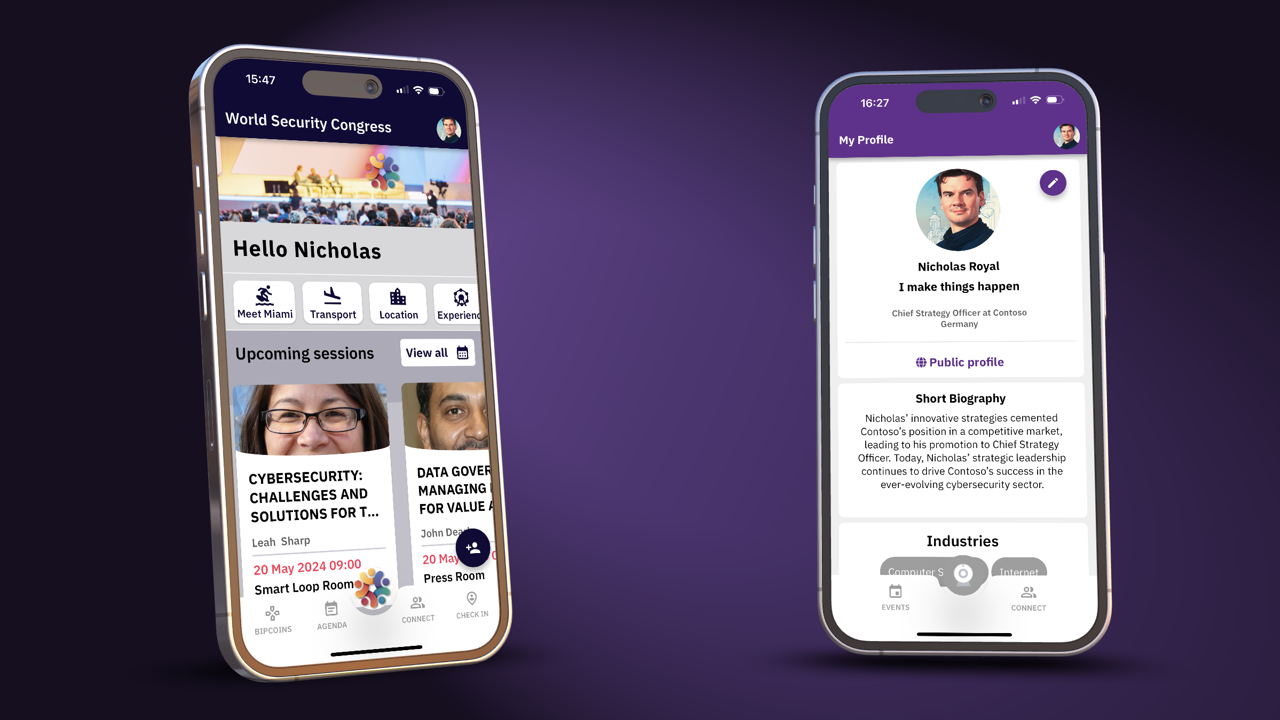
\includegraphics[width=1\linewidth]{slike/runevents-homeandprofile.png}
			\caption{Primjer početne stranice i stranice profila}
			\label{fig:home-profile}
		\end{figure}
		
		\begin{figure}
			\centering
			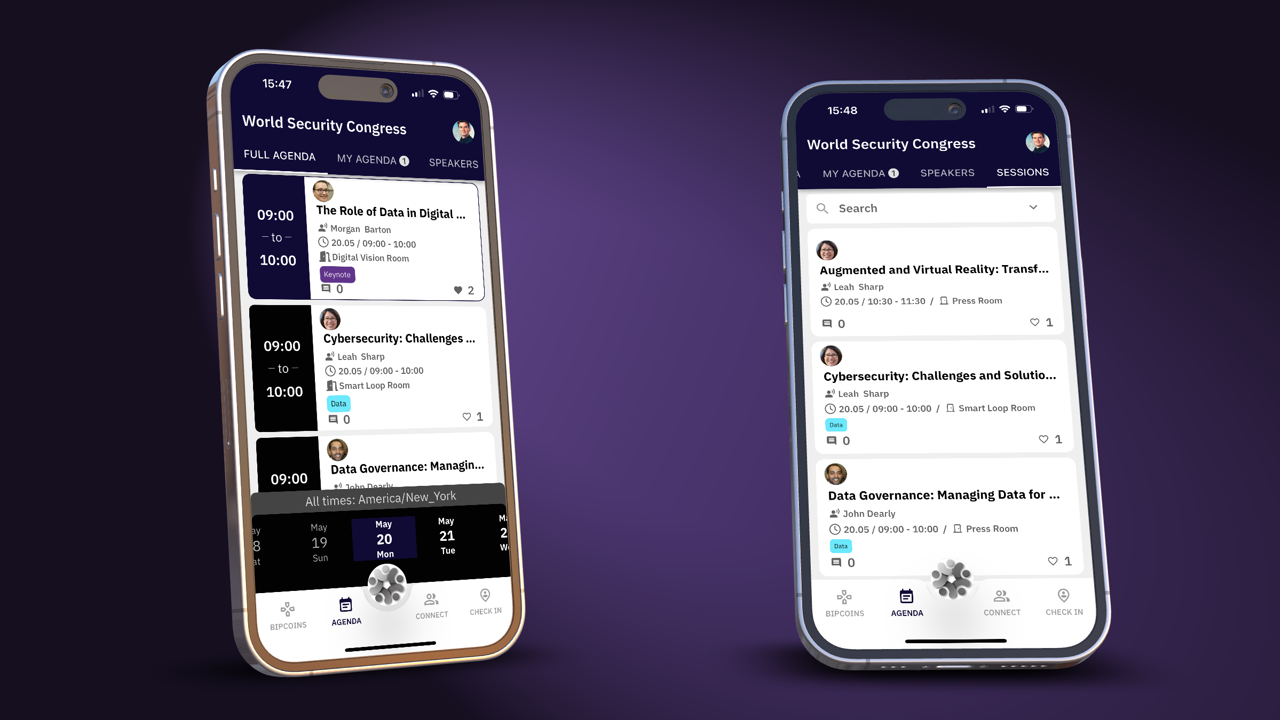
\includegraphics[width=1\linewidth]{slike/runevents-agenda.png}
			\caption{Primjer stranice za agendu i sesije}
			\label{fig:agenda-sessions}
		\end{figure}
		
		\begin{figure}
			\centering
			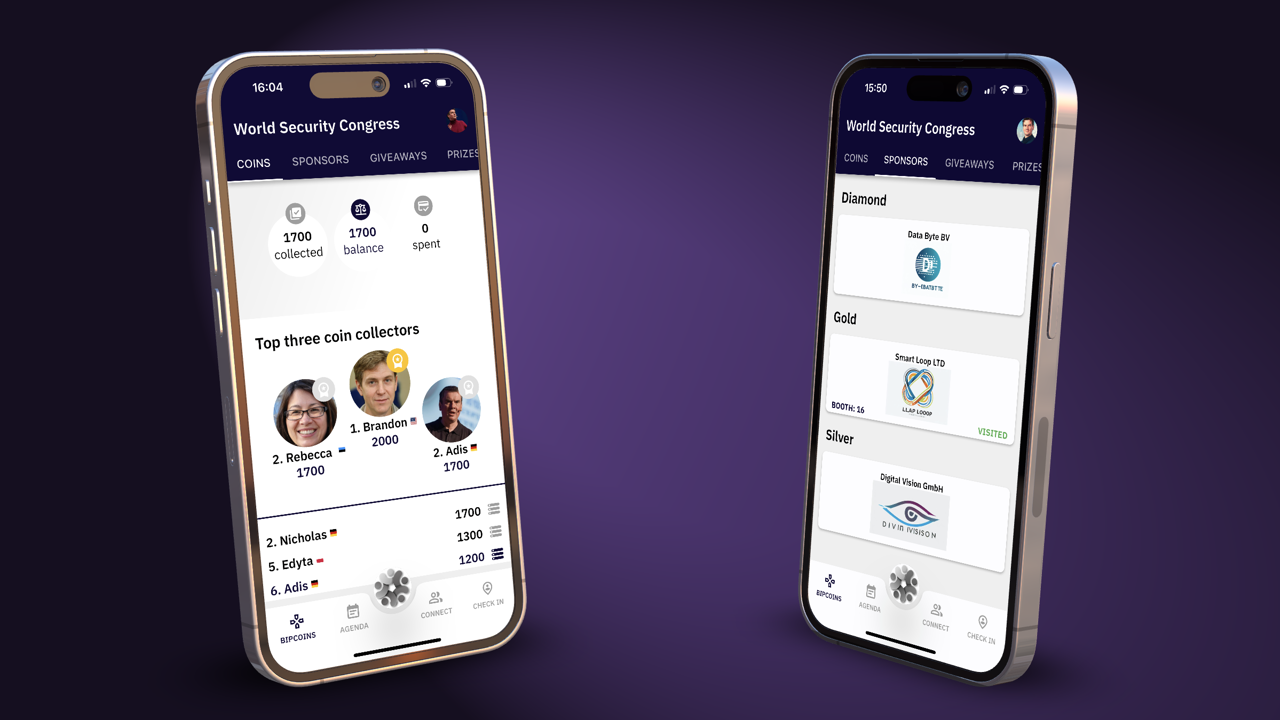
\includegraphics[width=1\linewidth]{slike/runevents-gameandsponsors.png}
			\caption{Primjer stranice za gamifikaciju i stranice sponzora}
			\label{fig:game-sponsors}
		\end{figure}
		
		\begin{figure}
			\centering
			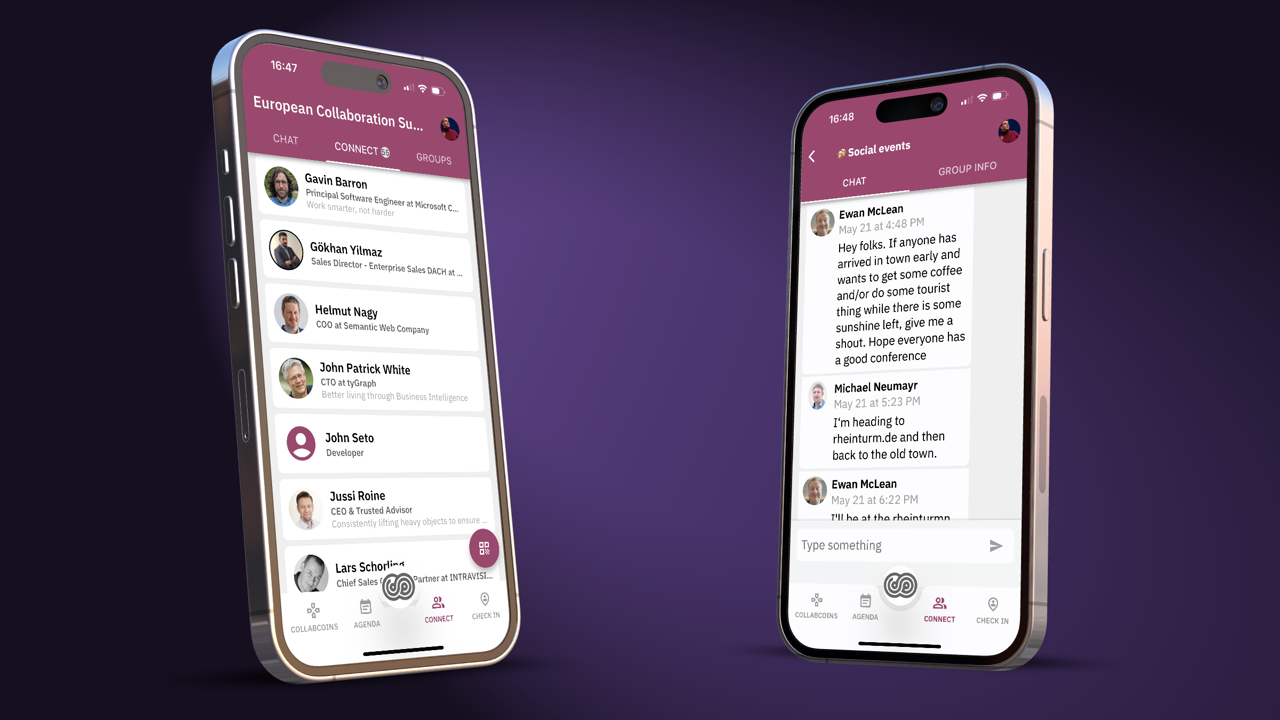
\includegraphics[width=1\linewidth]{slike/runevents-connectandchat.png}
			\caption{Primjer stranice za povezivanje i razgovor}
			\label{fig:connect-chat}
		\end{figure}
		
		\begin{figure}
			\centering
			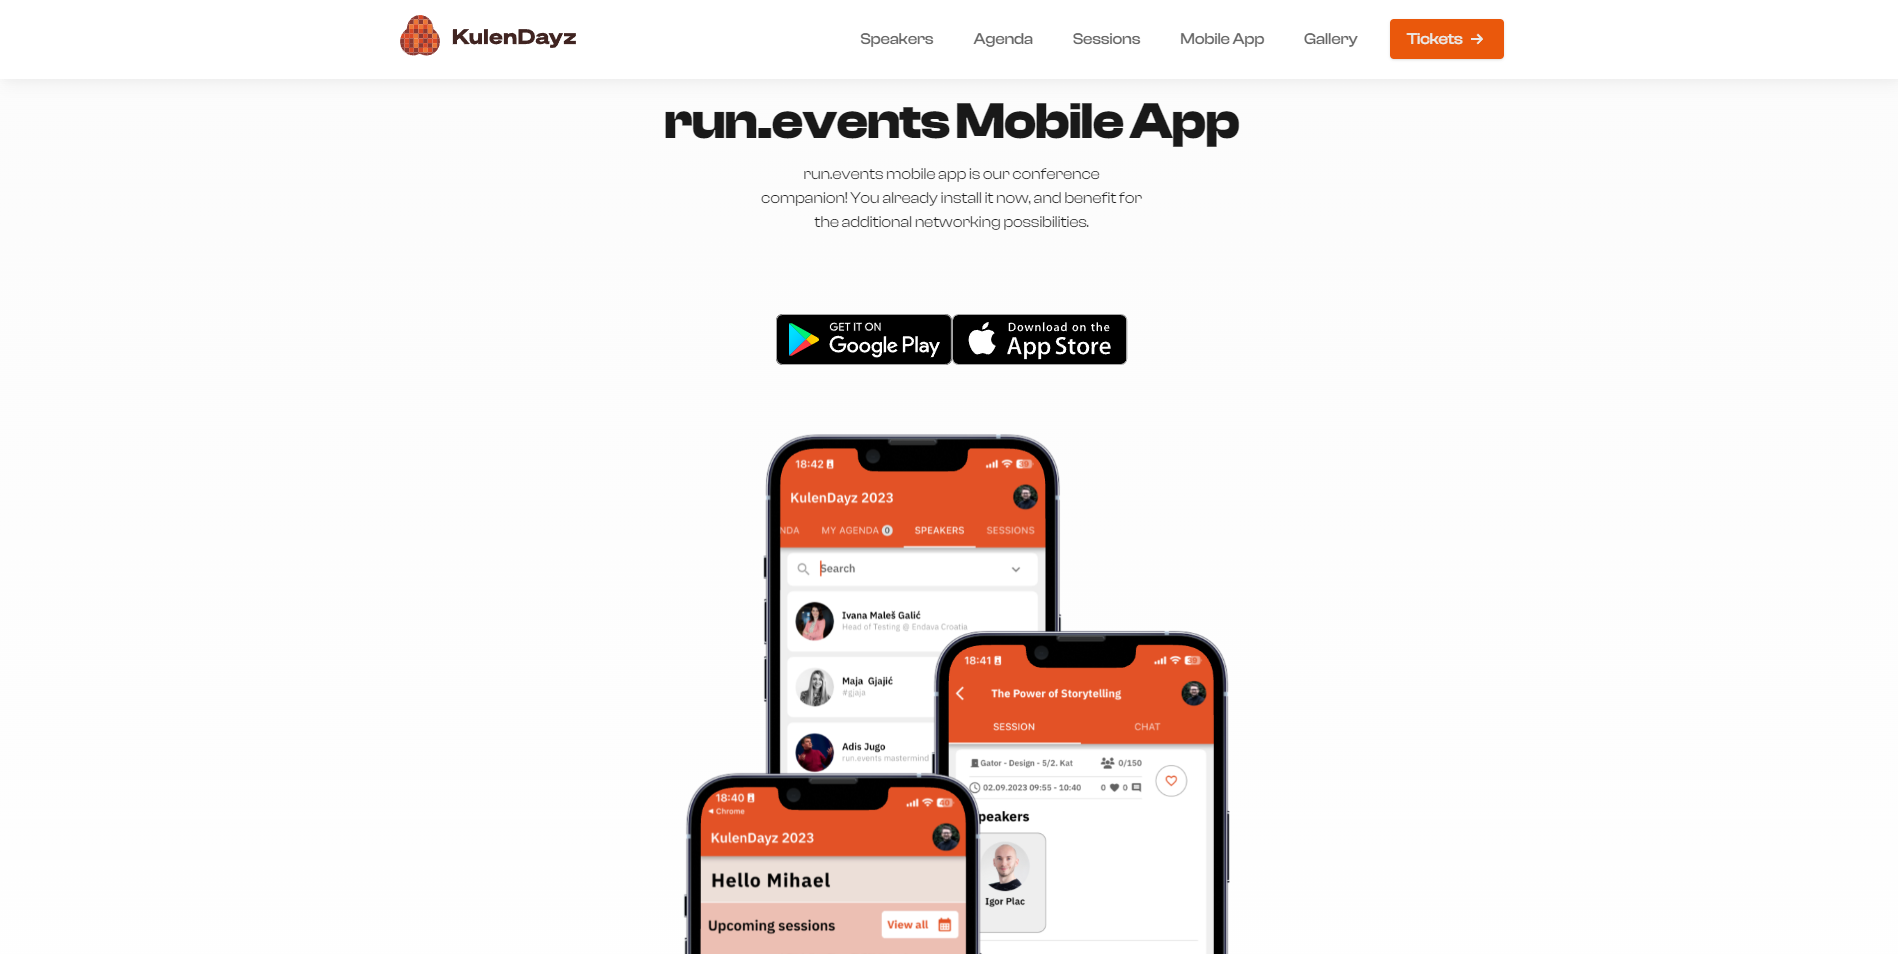
\includegraphics[width=1\linewidth]{kulen-runevents.png}
			\caption{Primjer stranice za instalaciju mobilne aplikacije \textit{run.events} u sklopu konferencije \textit{KulenDayz}}
			\label{fig:kulen-run}
		\end{figure}
		
		\begin{figure}
			\centering
			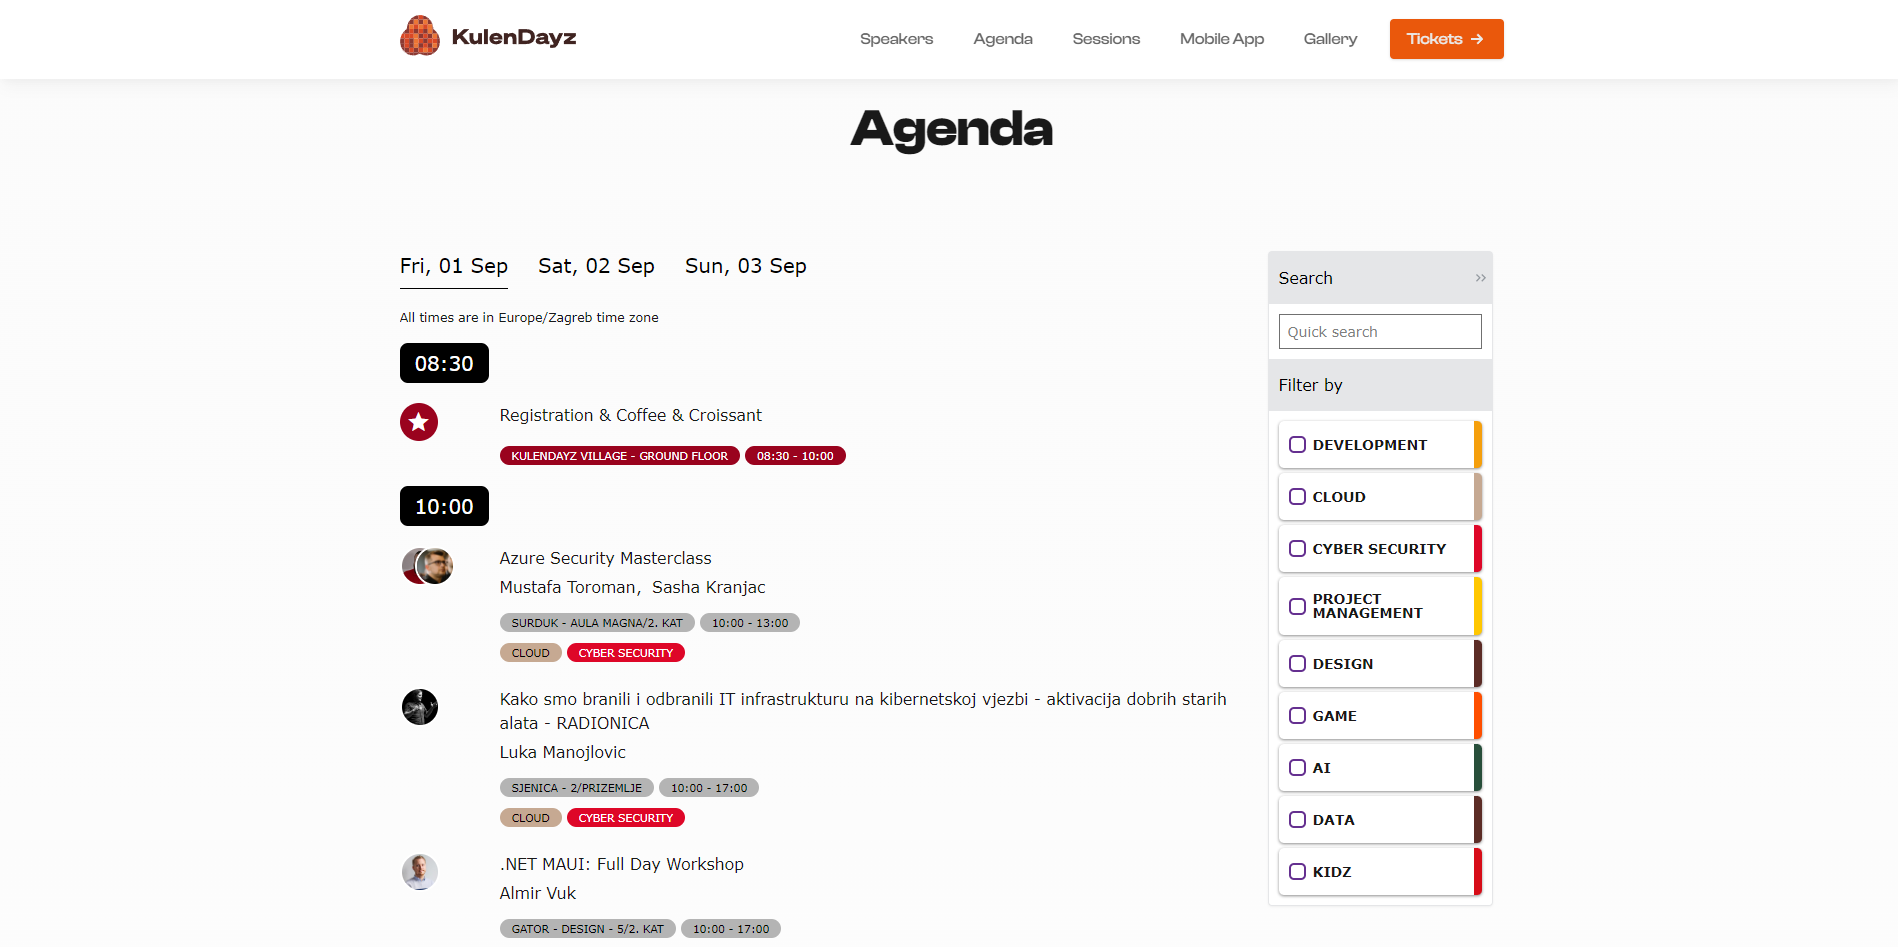
\includegraphics[width=1\linewidth]{slike/kulen-agenda.png}
			\caption{Primjer stranice za agendu implementirane iz \textit{run.events} koda}
			\label{fig:kulen-agenda}
		\end{figure}
		
		\begin{figure}
			\centering
			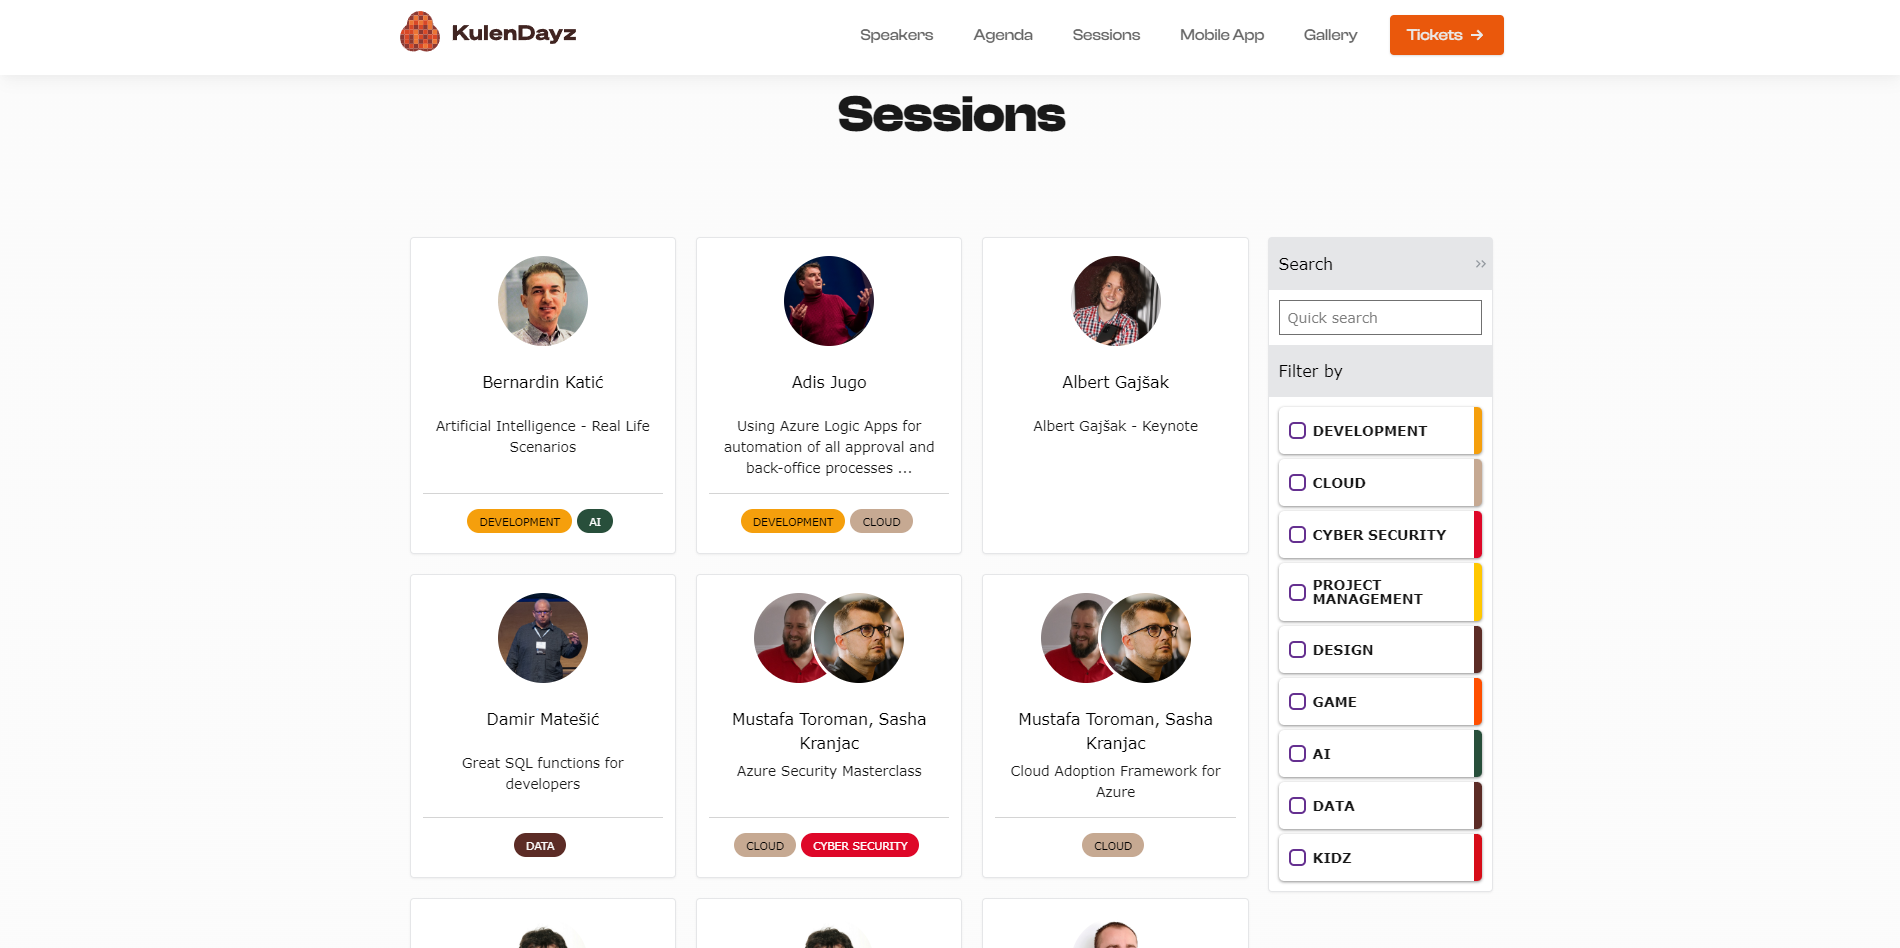
\includegraphics[width=1\linewidth]{slike/kulen-sessions.png}
			\caption{Primjer stranice za sesije implementirane iz \textit{run.events} koda}
			\label{fig:kulen-sessions}
		\end{figure}
		
		\begin{figure}
			\centering
			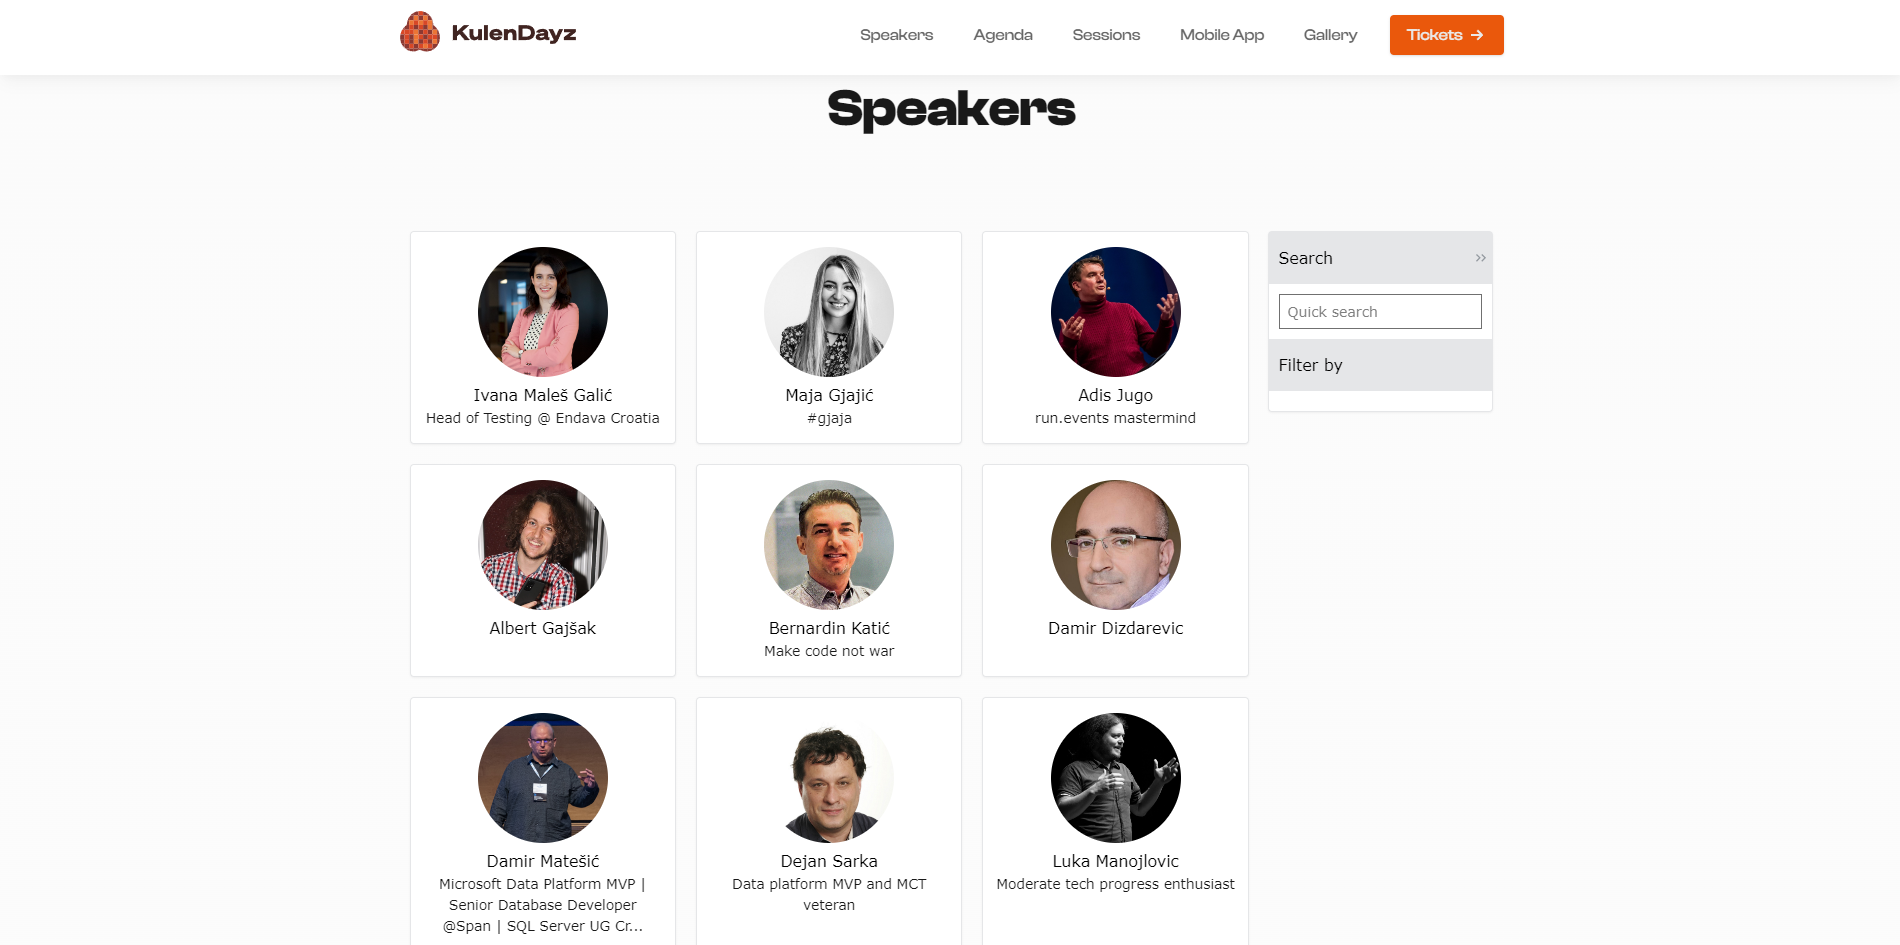
\includegraphics[width=1\linewidth]{slike/kulen-speakers.png}
			\caption{Primjer stranice za govornike implementirane iz \textit{run.events} koda}
			\label{fig:kulen-speakers}
		\end{figure}
		
		\eject
		
		\section{Primjeri u \LaTeX u}
		
		\textit{Ovo potpoglavlje izbrisati.}\\

		U nastavku se nalaze različiti primjeri kako koristiti osnovne funkcionalnosti \LaTeX a koje su potrebne za izradu dokumentacije. Za dodatnu pomoć obratiti se asistentu na projektu ili potražiti upute na sljedećim web sjedištima:
		\begin{itemize}
			\item Upute za izradu diplomskog rada u \LaTeX u - \url{https://www.fer.unizg.hr/_download/repository/LaTeX-upute.pdf}
			\item \LaTeX\ projekt - \url{https://www.latex-project.org/help/}
			\item StackExchange za Tex - \url{https://tex.stackexchange.com/}\\
		
		\end{itemize} 	


		
		\noindent \underbar{podcrtani tekst}, \textbf{podebljani tekst}, 	\textit{nagnuti tekst}\\
		\noindent \normalsize primjer \large primjer \Large primjer \LARGE {primjer} \huge {primjer} \Huge primjer \normalsize
				
		\begin{packed_item}
			
			\item  primjer
			\item  primjer
			\item  primjer
			\item[] \begin{packed_enum}
				\item primjer
				\item[] \begin{packed_enum}
					\item[1.a] primjer
					\item[b] primjer
				\end{packed_enum}
				\item primjer
			\end{packed_enum}
			
		\end{packed_item}
		
		\noindent primjer url-a: \url{https://www.fer.unizg.hr/predmet/proinz/projekt}
		
		\noindent posebni znakovi: \# \$ \% \& \{ \} \_ 
		$|$ $<$ $>$ 
		\^{} 
		\~{} 
		$\backslash$ 
		
		
		\begin{longtblr}[
			label=none,
			entry=none
			]{
				width = \textwidth,
				colspec={|X[8,l]|X[8, l]|X[16, l]|}, 
				rowhead = 1,
			} %definicija širine tablice, širine stupaca, poravnanje i broja redaka naslova tablice
			\hline \SetCell[c=3]{c}{\textbf{naslov unutar tablice}}	 \\ \hline[3pt]
			\SetCell{LightGreen}IDKorisnik & INT	&  	Lorem ipsum dolor sit amet, consectetur adipiscing elit, sed do eiusmod  	\\ \hline
			korisnickoIme	& VARCHAR &   	\\ \hline 
			email & VARCHAR &   \\ \hline 
			ime & VARCHAR	&  		\\ \hline 
			\SetCell{LightBlue} primjer	& VARCHAR &   	\\ \hline 
		\end{longtblr}
		

		\begin{longtblr}[
				caption = {Naslov s referencom izvan tablice},
				entry = {Short Caption},
			]{
				width = \textwidth, 
				colspec = {|X[8,l]|X[8,l]|X[16,l]|}, 
				rowhead = 1,
			}
			\hline
			\SetCell{LightGreen}IDKorisnik & INT	&  	Lorem ipsum dolor sit amet, consectetur adipiscing elit, sed do eiusmod  	\\ \hline
			korisnickoIme	& VARCHAR &   	\\ \hline 
			email & VARCHAR &   \\ \hline 
			ime & VARCHAR	&  		\\ \hline 
			\SetCell{LightBlue} primjer	& VARCHAR &   	\\ \hline 
		\end{longtblr}
	


		
		
		%unos slike
		\begin{figure}[H]
			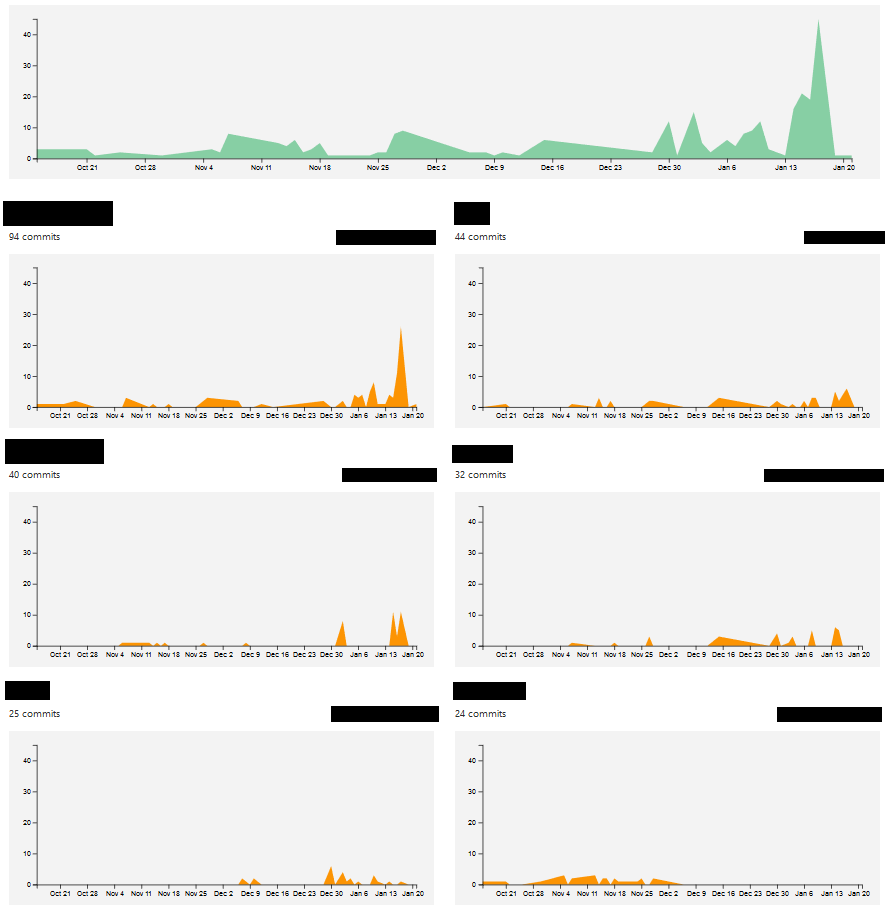
\includegraphics[scale=0.4]{slike/aktivnost.PNG} %veličina slike u odnosu na originalnu datoteku i pozicija slike
			\centering
			\caption{Primjer slike s potpisom}
			\label{fig:promjene}
		\end{figure}
		
		\begin{figure}[H]
			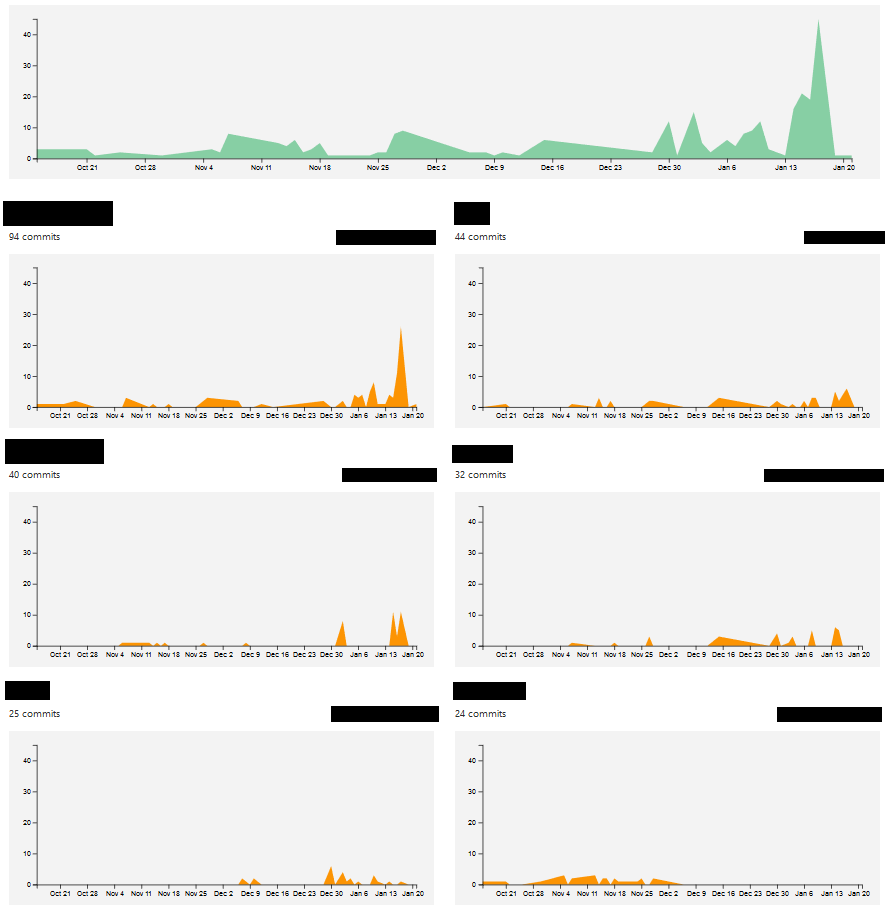
\includegraphics[width=\textwidth]{slike/aktivnost.PNG} %veličina u odnosu na širinu linije
			\caption{Primjer slike s potpisom 2}
			\label{fig:promjene2} %label mora biti drugaciji za svaku sliku
		\end{figure}
		
		Referenciranje slike \ref{fig:promjene2} u tekstu.
		
		\eject
		
	